\chapter{Anforderungen}

\section{Benutzer und Personas}


Die Benutzer der Project Helin Plattform teilen sich in zwei Gruppen auf, welche in dieser Arbeit berücksichtigt werden.

\subsection{Service-Nutzer}

Service-Nutzer verwenden nur die Service App um einen Service oder ein Gut an ihre Position zu bestellen. 

\subsubsection{Persona Diego}

\begin{figure}
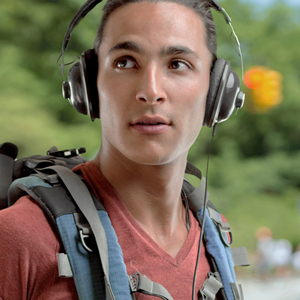
\includegraphics[width=.35\textwidth]{images/persona-diego.jpg} 
\caption{Persona Diego: Freie Lizenz; Quelle }
	%\url{http://blog.placeit.net/free-avatar-pack/}}
\label{fig:diego}
\end{figure}

Er ist \textbf{23 Jahre alt} wohnt in einer WG in Uster.\\

Diego hat eine Informatik-Lehre mit BMS abgeschlossen und ist auf der Suche nach einer neuen beruflichen oder schulischen Herausforderung.

\paragraph{Technisches Verhalten} 

Arbeitet täglich acht Stunden mit dem PC. Nutzt gerne neue Technologien. Besitzt ein Android-Smartphone der neusten Generation. Die Android Updates macht er immer sofort. Interessiert sich für neue Technologien und sieht sich regelmässig Kickstarter Projekte an.\\ 

\paragraph{Ziele} 

Möchte sich weiterbilden und neue Herausforderungen finden. Möchte Neue Technologien entdecken und einsetzen.\\

\subsection{Administratoren}

Administratoren verwenden die Project Helin Plattform um eine Flotte von Drohnen zu verwalten. Sie nutzen dazu die Webseite der Plattform und kümmern sich um das definieren von Flugzonen, Services und Gütern.

\subsubsection{Persona Stefanie}
\begin{figure}
	
\includegraphics[width=.35\textwidth]{images/persona-stefanie.jpg} 
	\caption{Persona Stefanie: Freie Lizenz; Quelle} %\url{http://blog.placeit.net/free-avatar-pack/}}
	\label{fig:stefanie}
\end{figure}


Carmen ist \textbf{35 Jahre alt} und lebt alleine in Zürich.

Sie unternimmt viel mit Freunden und reist gerne. Sie ist auf dem Land aufgewachsen und wohnt jetzt in Zürich. 

Carmen arbeitet bei einer Eventagentur und hat eine Ausbildung als Eventmanagerin abgeschlossen.

\paragraph{Technisches Verhalten} 
Sie nutzt den PC täglich bei der Arbeit, vor allem Planungstools und das E-Mail-Programm. Ausserdem ist sie zu Recherchezwecken viel im Internet unterwegs. Sie nutzt Chrome als Browser im Geschäft. Sie besitzt ein Samsung Galaxy S4, dass sie schon seit einigen Jahren verwendet. Zuhause hat sie keinen PC.

\paragraph{Kommunikationsverhalten}
Sie kommuniziert geschäftlich hauptsächlich per E-Mail. Mit Freunden kommuniziert sie über WhattsApp.

\paragraph{Ziele} 
Sie möchte mit neuen und innovativen Ideen Events für Besucher spannender gestalten.

\section{User-Stories}

Die funktionalen Anforderungen leiten sich aus der Aufgabenstellung, sowie den mit dem Betreuer diskutierten Ideen ab. 

\subsection{Administrator}
\begin{itemize}
\item Ich als Administrator kann auf der Webseite einen Account erstellen.
\item Ich als Administrator kann ein Projekt erfassen.
\item Ich als Administrator kann auf eine Drohne dem Projekt hinzufügen.
\item Ich als Administrator kann alle Drohnen verwalten (RUD).
\item Ich als Administrator kann Güter verwalten (CRUD).
\item Ich als Administrator kann Services verwalten (CRUD) (optional).
\item Ich als Administrator kann Flug-, Lade- und Abwurfzonen verwalten.
\item Ich als Administrator kann Bestellungen verwalten (CRUD).
\item Ich als Administrator kann Missionen vor, nach, und während der Ausführung ansehen.
\item Ich als Administrator kann Missionen abbrechen.
\end{itemize}

\subsection{Service-Nutzer}
\begin{itemize}
\item Ich als Service-Nutzer kann eine App aus dem Google Play Store herunterladen.
\item Ich als Service-Nutzer kann die App nutzen ohne mich anzumelden.
\item Ich als Service-Nutzer kann in der App aus einer Auswahl von Gütern und Services eine Auswahl treffen.
\item Ich als Service-Nutzer kann eine Bestellung tätigen.
\item Ich als Service-Nutzer kann auf der Karte des Smartphones die Bewegung der Drohne verfolgen.
\item Ich als Service-Nutzer erhalte textuelle Updates über den Status meiner Bestellung.
\item Ich als Service-Nutzer kann eine Bestellung stornieren.
\end{itemize}
